\documentclass[SEC,english,beameralt]{tumbeamer}

% If you load additional packages, do so in packages.sty as figures are build
% as standalone documents and you may want to have effect on them, too.

% Folder structure:
% .
% ├── beamermods.sty                  % depricated an will be removed soon
% ├── compile                         % remotely compile slides
% ├── figures                         % all figures go here
% │   └── schichtenmodelle_osi.tikz   % each .tikz or .tex is a target
% ├── include                         % create your document here
% │   ├── example.tex                 % example document
% │   └── slides.tex                  % make document wide changes here
% ├── lit.bib                         % literature
% ├── Makefile
% ├── moeptikz.sty                    % fancy networking symbols
% ├── packages.sty                    % load additional packages there
% ├── pics                            % binary pcitures go here
% ├── slides.tex                      % main document (may be more than one)
% ├── tumbeamer.cls
% ├── tumcolor.sty                    % TUM color definitions
% ├── tumcontact.sty                  % TUM headers and footers
% ├── tumlang.sty                     % TUM names and language settings
% └── tumlogo.sty                     % TUM logos

% Configure author, title, etc. here:
\usepackage[utf8]{inputenc}
\usepackage{packages}
\usepackage{beamermods}

% For beamer mode (default):
\author[Yiyang Xie]{Yiyang Xie}
\title[Web of Trust vs. PKI: A Survey on Trust Optimizations]{Web of Trust vs. PKI: A Survey on Trust Optimizations}

% Uncomment to add advisors for presentation in Oberseminar
\advisor{Maximilian Tschirschnitz}

% Uncomment to add type for presentation in Oberseminar
% Usage: \thesistype{intermediate | final}{bachelor | master | idp | gr}
%\thesistype{intermediate}{gr}

% Uncomment to configure date in dd-mm-yyyy format
\newdate{date}{01}{02}{2024}
\date{\displaydate{date}}

% Uncomment to add a venue to the title slide
%\venue{International Conference on Conferencing 2018 \\ Garching b. München, Germany}

% For lecture mode (use package option 'lecture'):
%\lecture[GRNVS]{Grundlagen Rechnernetze und Verteilte Systeme}
%\module{IN0010}
%\semester{SoSe\,2016}
%\assistants{Johannes Naab, Stephan Günther, Maurice Leclaire}


\usepackage{pgfpages}
\usepackage{ifthen}
% ============================================================================
% jobname solution
% ============================================================================
\newif\ifsolution%
\ifthenelse{\equal{\detokenize{notes}}{\jobname}}{%
    \setbeameroption{show notes on second screen=bottom}
    \setbeamercolor{note page}{bg=white, fg=black}
    \setbeamercolor{note title}{bg=white!95!black, fg=black}
}{
}

% TeXLive 2018 compatibility: https://tex.stackexchange.com/questions/426088/texlive-pretest-2018-beamer-and-subfig-collide
\makeatletter
\let\@@magyar@captionfix\relax
\makeatother


\begin{document}

% If you are preparing a talk but do not like the default font sizes, you may
% want to try the class option 'beameralt', which uses smaller default font
% sizes and integrates subsection/subsubsection names into the headline.

% For lecture mode, you may want to build one set of slides per chapter but
% with common page numbering. If so,
% 1) create a new .tex file for each chapter, e.g. slides_chapN.tex,
% 2) set the part counter to N-1 (assuming chapters start at 0), and
% 3) and name your chapter by using the \part{} command.
%\setcounter{part}{-1}
%\part{Organisatorisches und Einleitung}

% For 16:9 slides, use the class option 'aspectratio=169'.

% If class option 'noframenumbers' is given, frame numbers are not printed.

% If class option 'notitleframe' is given, the title frame is not autmatically
% generated.

% Class option 'nocontentframes' suppresses automatic generation of content
% frames when new parts/sections are started.

% Include source files from ./include (or ./include/chapN).
\section{Table of contents}
% 2
\begin{frame}
    \begin{itemize}
        \item<1> Definition of Latency
        \item<1> Introduction of Virtualization Technologies
            \begin{itemize}
                \item<1> Virtual Machines
                \item<1> Containers
            \end{itemize}
        \item<1> Requirements for Measurement
        \item<1> Methods of optimizing latency
        \item<1> Conclusion
    \end{itemize}
\end{frame}

\section{Definition of Latency}
% 8
\begin{frame}
    \centering
    \begin{itemize}
        \item magic triangle of 5G
              \begin{itemize}
                  \item enhanced Mobile BroadBand (eMBB)
                  \item massive Machine-Type Communication (mMTC)
                  \item \textbf{Ultra-Reliable and Low-Latency Communication (URLLC)}
              \end{itemize}
    \end{itemize}




    \begin{tabular}{|c|c|c|}
        \hline
        \textbf{URLLC Performance Metric} & \textbf{Minimal Value} & \textbf{Maximum Value} \\ \hline
        User plane latency (URLLC)        & -                      & 1ms                    \\ \hline
        Reliability (URLLC)               & 99.999\%               & -                      \\ \hline
    \end{tabular}

    \footnote{Minimum requirements related to technical performance
        for IMT-2020 radio interface(s), ITU, 2017 \cite{b1}}

\end{frame}



\section{Introduction of Virtualization Technologies}
% 11
\begin{frame}
    \centering
    \begin{figure}[h!]
        \centering
        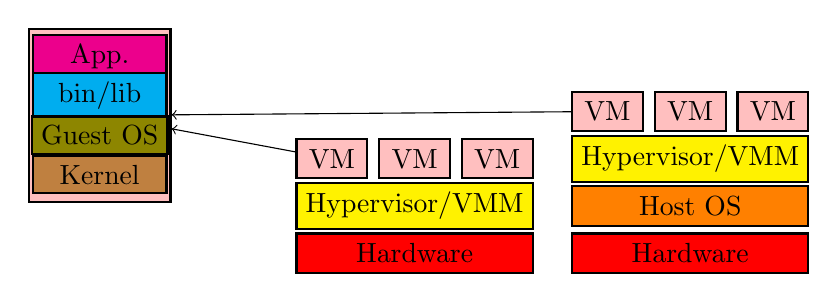
\begin{tikzpicture}
            \node [draw, thick, fill = pink, minimum width = 1.8cm, minimum height = 2.2cm]
            (vm)at(-3,2.75){};
            %App
            \node [draw, thick, fill = magenta, minimum width = 1.7cm, minimum height = 0.4cm]
            (va)at(-3,3.5){App.};
            %Bins/Lib
            \node [draw, thick, fill = cyan, minimum width = 1.7cm, minimum height = 0.4cm]
            (vb)at(-3,3){bin/lib};
            %Guest OS
            \node [draw, thick, fill = olive, minimum width = 1.7cm, minimum height = 0.4cm]
            (OS1)at(-3,2.5){Guest\ OS};
            %Kernel
            \node [draw, thick, fill = brown, minimum width = 1.7cm, minimum height = 0.4cm]
            (K1)at(-3,2){Kernel};

            %VM
            \node [draw, thick, fill = pink, minimum width = 0.9cm, minimum height = 0.5cm]
            (v1)at(-0.05,2.2){VM};
            \node [draw, thick, fill = pink, minimum width = 0.9cm, minimum height = 0.5cm]
            (v2)at(1,2.2){VM};
            \node [draw, thick, fill = pink, minimum width = 0.9cm, minimum height = 0.5cm]
            (v3)at(2.05,2.2){VM};

            \node [draw, thick, fill = pink, minimum width = 0.9cm, minimum height = 0.5cm]
            (v4)at(3.45,2.8){VM};
            \node [draw, thick, fill = pink, minimum width = 0.9cm, minimum height = 0.5cm]
            (v5)at(4.5,2.8){VM};
            \node [draw, thick, fill = pink, minimum width = 0.9cm, minimum height = 0.5cm]
            (v6)at(5.55,2.8){VM};

            %Hypervisor
            \node [draw, thick, fill = yellow, minimum width = 3cm, minimum height = 0.5cm]
            (Hyper1)at(1,1.6){Hypervisor/VMM};
            \node [draw, thick, fill = yellow, minimum width = 3cm, minimum height = 0.5cm]
            (Hyper2)at(4.5,2.2){Hypervisor/VMM};

            \node [draw, thick, fill = orange, minimum width = 3cm, minimum height = 0.5cm]
            (HOS2)at(4.5,1.6){Host OS};

            \node [draw, thick, fill = red, minimum width = 3cm, minimum height = 0.5cm]
            (Infra1)at(1,1){Hardware};
            \node [draw, thick, fill = red, minimum width = 3cm, minimum height = 0.5cm]
            (Infra2)at(4.5,1){Hardware};

            \draw [->](v1)--(vm);
            \draw [->](v4)--(vm);

        \end{tikzpicture}
        \caption{Structure of VM}
        \label{Structure of VM}
    \end{figure}
    \begin{itemize}
        \item Hypervisor: Type 1 (without Host OS), Type 2 (with Host OS)
        \item VMs:
              \begin{itemize}
                  \item \textbf{with full Guest OS}
                  \item store traditional monolithic workloads,
                        e.g.\ abstracting, separating, replicating and emulating
                        entire servers, operating systems, desktops, databases and networks.
                        \footnote{Introduction to Virtualization, Brief History of Virtualization, oracle, 2012 \cite{b2}}
              \end{itemize}
    \end{itemize}
\end{frame}


\section{Introduction of Virtualization Technologies}
% 13
\begin{frame}
    \begin{figure}[h!]
        \centering
        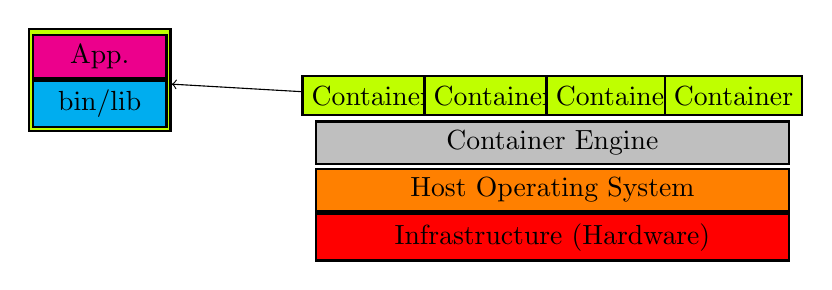
\begin{tikzpicture}
            \node [draw, thick, fill = lime, minimum width = 1.8cm, minimum height = 1.3cm]
            (cc)at(-3,2){};
            %App
            \node [draw, thick, fill = magenta, minimum width = 1.7cm, minimum height = 0.5cm]
            (ca)at(-3,2.3){App.};
            %Bins/Lib
            \node [draw, thick, fill = cyan, minimum width = 1.7cm, minimum height = 0.5cm]
            (cb)at(-3,1.7){bin/lib};
            %Container
            \node [draw, thick, fill = lime, minimum width = 1cm, minimum height = 0.5cm]
            (c1)at(0.45,1.8){Container};
            \node [draw, thick, fill = lime, minimum width = 1cm, minimum height = 0.5cm]
            (c2)at(2,1.8){Container};
            \node [draw, thick, fill = lime, minimum width = 1cm, minimum height = 0.5cm]
            (c3)at(3.55,1.8){Container};
            \node [draw, thick, fill = lime, minimum width = 1cm, minimum height = 0.5cm]
            (c4)at(5.05,1.8){Container};
            %Container Engine
            \node [draw, thick, fill = lightgray, minimum width = 6cm, minimum height = 0.5cm]
            (Hyper)at(2.75,1.2){Container Engine};
            \node [draw, thick, fill = orange, minimum width = 6cm, minimum height = 0.5cm]
            (HOS)at(2.75,0.6){Host Operating System};
            \node [draw, thick, fill = red, minimum width = 6cm, minimum height = 0.5cm]
            (Infra)at(2.75,0){Infrastructure (Hardware)};

            \draw [->](c1)--(cc);

        \end{tikzpicture}
        \caption{Structure of Container}
        \label{Structure of Container}
    \end{figure}
    \begin{itemize}
        \item Containers:
              \begin{itemize}
                  \item much smaller than VMs, \textbf{without the Guest OS}
                  \item encapsulate individual functions, i.e.\ microservices.
                        \footnote{Containers vs. Virtual Machines, microsoft, 2021 \cite{b3}}
              \end{itemize}
    \end{itemize}
\end{frame}

\section{Introduction of Virtualization Technologies}
% 15
\begin{frame}
    \centering
    \includegraphics<1>[width=.7\textwidth, page=1]{pics/Container}
    \footnote{[Online; accessed 24-Jan-2023] https://akfpartners.com/growth-blog/vms-vs-containers}
    \begin{itemize}
        \item VMs: more resources, more operations
        \item Containers: lightweight, high scalability, high portability
    \end{itemize}
\end{frame}

% 18
\section{Requirements for Measurement}
\begin{frame}
    \centering
    \includegraphics<1>[width=.6\textwidth, page=1]{pics/Acc&Pre2}
    \footnote{[Online; accessed 24-Jan-2023] https://sixsigmadsi.com/precision-and-accuracy/}
    \begin{itemize}
        \item Accuracy: the timestamp differences between measurement and occurrence
        \item Precision: the fluctuations between measurements
    \end{itemize}
\end{frame}

% 21
\section{Methods of optimizing latency}
\begin{frame}
    \centering
    \includegraphics<1>[width=.4\textwidth, page=1]{pics/Optimization2}
    \includegraphics<1>[width=.55\textwidth, page=1]{pics/Optimization1}
    \footnote{S. Gallenmüller, F. Wiedner, J. Naab, and G. Carle, “Ducked Tails:
        Trimming the Tail Latency of(f) Packet Processing Systems,” 17th
        International Conference on Network and Service Management
        (CNSM), 2021, p.537, 2021 \cite{b5}}
    \begin{itemize}
        \item Disable virtual cores
        \item Enable core isolation
        \item Reduce the number of CPU OS interrupts
        \item Disable energy saving mechanism
    \end{itemize}
\end{frame}

% 23
\section{Methods of optimizing latency}
\begin{frame}
    \centering
    \includegraphics<1>[width=.4\textwidth, page=1]{pics/Optimization3}
    \includegraphics<1>[width=.4\textwidth, page=1]{pics/Optimization4}
    \footnote{A. M. Joy, “Performance Comparison between Linux Containers
        and Virtual Machines,” International Conference on Advances in
        Computer Engineering and Applications, 2015, p. 342, 2015. \cite{b4}}
    \begin{itemize}
        \item Containers:
              \begin{itemize}
                  \item over 5 times requests more than VMs
                  \item great scalability, about 22 times of VMs
                        (high portability)
              \end{itemize}
    \end{itemize}
\end{frame}


% 25
\section{Conclusion}
\begin{frame}
    \begin{itemize}
        \item Virtualization: Running multiple independent systems simultaneously
        \item Differences between VMs \& Containers:
              \begin{itemize}
                  \item Isolation
                  \item Scalability
                  \item Portability
              \end{itemize}
        \item Current latency optimization is satisfactory
        \item Next step
              \begin{itemize}
                  \item Containers make it possible to optimize the latency continuously
                  \item Hybrid virtualization
              \end{itemize}
    \end{itemize}
\end{frame}


% Include markdown source from ./pandoc
%\section{Table of contents}
% 2
\begin{frame}
    \begin{itemize}
        \item<1> Definition of Latency
        \item<1> Introduction of Virtualization Technologies
            \begin{itemize}
                \item<1> Virtual Machines
                \item<1> Containers
            \end{itemize}
        \item<1> Requirements for Measurement
        \item<1> Methods of optimizing latency
        \item<1> Conclusion
    \end{itemize}
\end{frame}

\section{Definition of Latency}
% 8
\begin{frame}
    \centering
    \begin{itemize}
        \item magic triangle of 5G
              \begin{itemize}
                  \item enhanced Mobile BroadBand (eMBB)
                  \item massive Machine-Type Communication (mMTC)
                  \item \textbf{Ultra-Reliable and Low-Latency Communication (URLLC)}
              \end{itemize}
    \end{itemize}




    \begin{tabular}{|c|c|c|}
        \hline
        \textbf{URLLC Performance Metric} & \textbf{Minimal Value} & \textbf{Maximum Value} \\ \hline
        User plane latency (URLLC)        & -                      & 1ms                    \\ \hline
        Reliability (URLLC)               & 99.999\%               & -                      \\ \hline
    \end{tabular}

    \footnote{Minimum requirements related to technical performance
        for IMT-2020 radio interface(s), ITU, 2017 \cite{b1}}

\end{frame}



\section{Introduction of Virtualization Technologies}
% 11
\begin{frame}
    \centering
    \begin{figure}[h!]
        \centering
        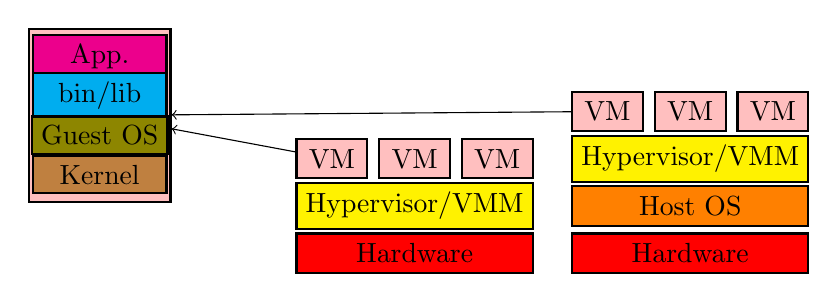
\begin{tikzpicture}
            \node [draw, thick, fill = pink, minimum width = 1.8cm, minimum height = 2.2cm]
            (vm)at(-3,2.75){};
            %App
            \node [draw, thick, fill = magenta, minimum width = 1.7cm, minimum height = 0.4cm]
            (va)at(-3,3.5){App.};
            %Bins/Lib
            \node [draw, thick, fill = cyan, minimum width = 1.7cm, minimum height = 0.4cm]
            (vb)at(-3,3){bin/lib};
            %Guest OS
            \node [draw, thick, fill = olive, minimum width = 1.7cm, minimum height = 0.4cm]
            (OS1)at(-3,2.5){Guest\ OS};
            %Kernel
            \node [draw, thick, fill = brown, minimum width = 1.7cm, minimum height = 0.4cm]
            (K1)at(-3,2){Kernel};

            %VM
            \node [draw, thick, fill = pink, minimum width = 0.9cm, minimum height = 0.5cm]
            (v1)at(-0.05,2.2){VM};
            \node [draw, thick, fill = pink, minimum width = 0.9cm, minimum height = 0.5cm]
            (v2)at(1,2.2){VM};
            \node [draw, thick, fill = pink, minimum width = 0.9cm, minimum height = 0.5cm]
            (v3)at(2.05,2.2){VM};

            \node [draw, thick, fill = pink, minimum width = 0.9cm, minimum height = 0.5cm]
            (v4)at(3.45,2.8){VM};
            \node [draw, thick, fill = pink, minimum width = 0.9cm, minimum height = 0.5cm]
            (v5)at(4.5,2.8){VM};
            \node [draw, thick, fill = pink, minimum width = 0.9cm, minimum height = 0.5cm]
            (v6)at(5.55,2.8){VM};

            %Hypervisor
            \node [draw, thick, fill = yellow, minimum width = 3cm, minimum height = 0.5cm]
            (Hyper1)at(1,1.6){Hypervisor/VMM};
            \node [draw, thick, fill = yellow, minimum width = 3cm, minimum height = 0.5cm]
            (Hyper2)at(4.5,2.2){Hypervisor/VMM};

            \node [draw, thick, fill = orange, minimum width = 3cm, minimum height = 0.5cm]
            (HOS2)at(4.5,1.6){Host OS};

            \node [draw, thick, fill = red, minimum width = 3cm, minimum height = 0.5cm]
            (Infra1)at(1,1){Hardware};
            \node [draw, thick, fill = red, minimum width = 3cm, minimum height = 0.5cm]
            (Infra2)at(4.5,1){Hardware};

            \draw [->](v1)--(vm);
            \draw [->](v4)--(vm);

        \end{tikzpicture}
        \caption{Structure of VM}
        \label{Structure of VM}
    \end{figure}
    \begin{itemize}
        \item Hypervisor: Type 1 (without Host OS), Type 2 (with Host OS)
        \item VMs:
              \begin{itemize}
                  \item \textbf{with full Guest OS}
                  \item store traditional monolithic workloads,
                        e.g.\ abstracting, separating, replicating and emulating
                        entire servers, operating systems, desktops, databases and networks.
                        \footnote{Introduction to Virtualization, Brief History of Virtualization, oracle, 2012 \cite{b2}}
              \end{itemize}
    \end{itemize}
\end{frame}


\section{Introduction of Virtualization Technologies}
% 13
\begin{frame}
    \begin{figure}[h!]
        \centering
        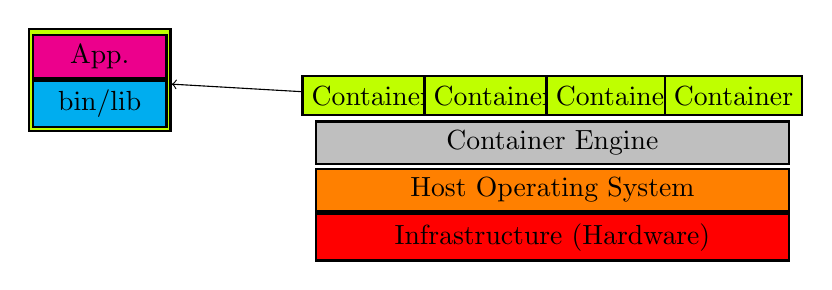
\begin{tikzpicture}
            \node [draw, thick, fill = lime, minimum width = 1.8cm, minimum height = 1.3cm]
            (cc)at(-3,2){};
            %App
            \node [draw, thick, fill = magenta, minimum width = 1.7cm, minimum height = 0.5cm]
            (ca)at(-3,2.3){App.};
            %Bins/Lib
            \node [draw, thick, fill = cyan, minimum width = 1.7cm, minimum height = 0.5cm]
            (cb)at(-3,1.7){bin/lib};
            %Container
            \node [draw, thick, fill = lime, minimum width = 1cm, minimum height = 0.5cm]
            (c1)at(0.45,1.8){Container};
            \node [draw, thick, fill = lime, minimum width = 1cm, minimum height = 0.5cm]
            (c2)at(2,1.8){Container};
            \node [draw, thick, fill = lime, minimum width = 1cm, minimum height = 0.5cm]
            (c3)at(3.55,1.8){Container};
            \node [draw, thick, fill = lime, minimum width = 1cm, minimum height = 0.5cm]
            (c4)at(5.05,1.8){Container};
            %Container Engine
            \node [draw, thick, fill = lightgray, minimum width = 6cm, minimum height = 0.5cm]
            (Hyper)at(2.75,1.2){Container Engine};
            \node [draw, thick, fill = orange, minimum width = 6cm, minimum height = 0.5cm]
            (HOS)at(2.75,0.6){Host Operating System};
            \node [draw, thick, fill = red, minimum width = 6cm, minimum height = 0.5cm]
            (Infra)at(2.75,0){Infrastructure (Hardware)};

            \draw [->](c1)--(cc);

        \end{tikzpicture}
        \caption{Structure of Container}
        \label{Structure of Container}
    \end{figure}
    \begin{itemize}
        \item Containers:
              \begin{itemize}
                  \item much smaller than VMs, \textbf{without the Guest OS}
                  \item encapsulate individual functions, i.e.\ microservices.
                        \footnote{Containers vs. Virtual Machines, microsoft, 2021 \cite{b3}}
              \end{itemize}
    \end{itemize}
\end{frame}

\section{Introduction of Virtualization Technologies}
% 15
\begin{frame}
    \centering
    \includegraphics<1>[width=.7\textwidth, page=1]{pics/Container}
    \footnote{[Online; accessed 24-Jan-2023] https://akfpartners.com/growth-blog/vms-vs-containers}
    \begin{itemize}
        \item VMs: more resources, more operations
        \item Containers: lightweight, high scalability, high portability
    \end{itemize}
\end{frame}

% 18
\section{Requirements for Measurement}
\begin{frame}
    \centering
    \includegraphics<1>[width=.6\textwidth, page=1]{pics/Acc&Pre2}
    \footnote{[Online; accessed 24-Jan-2023] https://sixsigmadsi.com/precision-and-accuracy/}
    \begin{itemize}
        \item Accuracy: the timestamp differences between measurement and occurrence
        \item Precision: the fluctuations between measurements
    \end{itemize}
\end{frame}

% 21
\section{Methods of optimizing latency}
\begin{frame}
    \centering
    \includegraphics<1>[width=.4\textwidth, page=1]{pics/Optimization2}
    \includegraphics<1>[width=.55\textwidth, page=1]{pics/Optimization1}
    \footnote{S. Gallenmüller, F. Wiedner, J. Naab, and G. Carle, “Ducked Tails:
        Trimming the Tail Latency of(f) Packet Processing Systems,” 17th
        International Conference on Network and Service Management
        (CNSM), 2021, p.537, 2021 \cite{b5}}
    \begin{itemize}
        \item Disable virtual cores
        \item Enable core isolation
        \item Reduce the number of CPU OS interrupts
        \item Disable energy saving mechanism
    \end{itemize}
\end{frame}

% 23
\section{Methods of optimizing latency}
\begin{frame}
    \centering
    \includegraphics<1>[width=.4\textwidth, page=1]{pics/Optimization3}
    \includegraphics<1>[width=.4\textwidth, page=1]{pics/Optimization4}
    \footnote{A. M. Joy, “Performance Comparison between Linux Containers
        and Virtual Machines,” International Conference on Advances in
        Computer Engineering and Applications, 2015, p. 342, 2015. \cite{b4}}
    \begin{itemize}
        \item Containers:
              \begin{itemize}
                  \item over 5 times requests more than VMs
                  \item great scalability, about 22 times of VMs
                        (high portability)
              \end{itemize}
    \end{itemize}
\end{frame}


% 25
\section{Conclusion}
\begin{frame}
    \begin{itemize}
        \item Virtualization: Running multiple independent systems simultaneously
        \item Differences between VMs \& Containers:
              \begin{itemize}
                  \item Isolation
                  \item Scalability
                  \item Portability
              \end{itemize}
        \item Current latency optimization is satisfactory
        \item Next step
              \begin{itemize}
                  \item Containers make it possible to optimize the latency continuously
                  \item Hybrid virtualization
              \end{itemize}
    \end{itemize}
\end{frame}


% Comment out if you do not want a bibliography
\section{Bibliography}
\begin{frame}[allowframebreaks]
    \bibliographystyle{abbrv}
    \setbeamertemplate{bibliography item}[text]
    \footnotesize
    \bibliography{lit}
\end{frame}

\end{document}

